\documentclass[BoSSSForSolvingConservationLaws.tex]{subfiles}

\begin{document}
For integrations involving nonlinear equation components of codomain variables we need to know the quadrature type (Volume, Edge or ...), number of integrals\coderm{BoSSS.Foundation.Quadrature.NonLin.NECQuadratureCommon.NoOfIntegrals(...)} ($N_{integrals}=\sum_{\gamma=0}^{\Gamma-1} N_{P\gamma}$ for Volume and $N_{integrals}=2\sum_{\gamma=0}^{\Gamma-1} N_{P\gamma}$ for Edge) and the required precision for integration\coderm{BoSSS.Foundation.Quadrature.NonLin.NECQuadratureCommon.FindQuadratureOder(...)}. Number of integrals are used for allocating memory required for the quadrature. A map, $MyMap(\gamma,m)$\coderm{BoSSS.Foundation.Quadrature.FluxQuadCommon.MyMap()}, is defined\coderm{BoSSS.Foundation.Quadrature.NonLin.NECQuadratureCommon.NECQuadratureCommon(...)} that provides index for the integral corresponding to codomain variable (equation) $\gamma$ and test function $m$. This index is the same for all cells because the same arrangement of codomain variables and test functions is considered for the cells (see section \ref{sec:CoordinateMapping}, \nameref{sec:CoordinateMapping}).\\
For computing integrals of nonlinear equation components there is no difference between parameters and domain variables, because domain variables are also known and taken from the previous time step or initial data. Therefore parameters are added\coderm{BoSSS.Foundation.Quadrature.NonLin.NECQuadratureCommon.NECQuadratureCommon(...)} at the end of domain variables' list. Moreover equation components of the type nonlinear flux\coderm{BoSSS.Foundation.INonlinearFlux} are sorted\coderm{BoSSS.Foundation.Quadrature.FluxQuadCommon.EquationComponentArgMapping.EquationComponentArgMapping(...)} for all codomain variables.\\
Referring to the general quadrature described at sec \ref{sec:QuadRules}, followings are some details of the execution procedure specific to nonlinear volume and edge quadratures. However for both volume and edge quadratures we must find\coderm{BoSSS.Foundation.Grid.GridData.TransformLocal2Global(...)} global coordinates\coderm{BoSSS.Foundation.Quadrature.NonLin.NECQuadratureCommon.m\_NodesGlobalCoords} (See section \ref{sec:Element-wise operations},\\ \nameref{sec:Element-wise operations}) of the quadrature points to calculate fluxes or sources. At the end results of integration of nonlinear equation components are accumulated in $m\_Output$\coderm{BoSSS.Foundation.Quadrature.NonLin.NECQuadratureCommon.m\_Output} which is a $1D$ array of doubles. Index to this array corresponds to the coordinate mapping of codomain variables.

\subsection{Nonlinear volume quadrature}
A volume quadrature computes integrals like $-\int_{K_j} [\vec{f}_j^h\cdot \nabla \phi_{jm} - q_j^h \phi_{jm}] d\vec{x}, \quad 0\leq m \leq N_p-1$ for a scalar conservation law, in all cells. When a volume quadrature is created\coderm{BoSSS.Foundation.Quadrature.NonLin.NECQuadratureVolume.NECQuadratureVolume(...)} equation components of type nonlinear source are also sorted for all codomain variables. Followings are details of general quadrature specific to nonlinear volume quadrature.
\begin{itemize}
\item \textbf{Creating node set family}\\
The node set family has only one set of nodes which are quadrature points\coderm{BoSSS.Foundation.Quadrature.Quadrature.\_QuadRule.Nodes} of the quadrature rule.
\item \textbf{Specifying memory}\\
Besides the memory required for the general quadrature, memory is allocated\coderm{BoSSS.Foundation.Quadrature.NonLin.NECQuadratureVolume.AllocateBuffers(...)} for field, flux and source values.
\item \textbf{Finding values of test functions and gradient of test functions}\\
Values of the test functions\coderm{BoSSS.Foundation.Basis.Evaluate(...)} and gradient of test functions\coderm{BoSSS.Foundation.Basis.EvaluateGradient(...)} are found\coderm{BoSSS.Foundation.Quadrature.Quadrature.PostLockNodes(...)} at the node set family and stored at $m\_TestFunctions[\gamma][n\_node, m]$ and\\ $m\_GradientTestFunctions[\gamma][n\_node, m, d]$. $d$\nomenclature{$d$}{Index for spatial dimension} is index for spatial dimension.
\item \textbf{Evaluation of integrands}\\
For a volume quadrature the integrand is $\vec{f}_j^h\cdot \nabla \phi_{jm}-q_j^h \phi_{jm}$ to be evaluated.
\begin{enumerate}
\item \textbf{Evaluation of domain and parameters variables}\\
Fields\coderm{BoSSS.Foundation.CoordinateMapping.Fields} in the domain coordinate mapping (including parameters) are evaluated at the node set and the result is $m\_FieldValues[f][j,n\_node]$. This is an array of 2D arrays used for evaluating each field $f$ in cell $j$ and node $n\_node$ of the node set.
\item \textbf{Transform nodes to global coordinates}\\
Global coordinates of the nodes of the only node set in the node set family \\$NodesUntransformed[n\_node,d]$ are found and stored at \\$m\_NodesGlobalCoords[j,n\_node,d]$.
\item \textbf{Evaluating flux functions}\\
flux functions of all equation components of type nonlinear flux corresponding to codomain variable $\gamma$ are calculated\coderm{BoSSS.Solution.Utils.NonlinearFlux.Flux(...)} and accumulated at \\$m\_FluxValues[\gamma][j,n\_node,d]$.
\item \textbf{Evaluating sources}\\
All equation components of type nonlinear source corresponding to codomain variable $\gamma$ are calculated\coderm{BoSSS.Foundation.INonlinearSource.Source(...)} and accumulated at $m\_SourceValues[\gamma][j, n\_node]$.
\item \textbf{Multiplying fluxes by gradient of test functions}\\
Flux values $m\_FluxValues[\gamma][j,n\_node,d]$ are multiplied by the transpose of inverse transformation matrix $((M_j)^{-1})^T$ of cell $j$ and scaled (see section \ref{sec:Element-wise operations}). Then they are multiplied by the value of gradient of the test functions \\$m\_GradientTestFunctions[\gamma][n\_node, m, d]$ and accumulated at \\$EvalResult[j, n\_node, MyMap(\gamma, m)]$, the evaluation results of integrands.
\item \textbf{Multiplying sources by test functions}\\
Source values $m\_SourceValues[\gamma][j, n\_node]$ are multiplied by the test functions $m\_TestFunctions[\gamma][n\_node, m]$ and subtracted from $EvalResult[j, n\_node, MyMap(\gamma, m)]$.
\end{enumerate}
\item \textbf{Saving integration results}\\
After integrating (see section \ref{sec:QuadRules}, \nameref{sec:QuadRules}) the quadrature results of a volume quadrature, $ResultsOfIntegration[j, MyMap(\gamma, m)]$ are subtracted from the output of the nonlinear quadrature, \\$m\_Output[m\_CodomainMapping.LocalUniqueCoordinateIndex(\gamma, j, m)]$.
\end{itemize}

\subsection{Nonlinear edge quadrature}
An edge quadrature computes integrals like the following for a scalar conservation law for all edges $i$, $0\leq i \leq (NoOfEdges-1)$\coderm{BoSSS.Foundation.Grid.GridData.NoOfEdges}.
\begin{align*}
 \int_{E_i} \hat{n}\cdot \vec{f}_j^* \phi_{jm} d\vec{x}, \qquad &0\leq m \leq N_p-1\\
 &E_i \in \partial K_j
\end{align*}
Because values of the integrals depend on test functions of the neighbor elements, two integrals must be computed for each edge considering both the first and second (if it exists) neighbors. As a result, number of integrals for an edge quadrature is twice of a volume quadrature. Details of a nonlinear edge quadrature is as follows.

\begin{itemize}
\item \textbf{Creating node set family}\\
When the quadrature type is Edge, quadrature points are points defined in coordinate system of the edge simplex but nodes of a node set must be defined in the volume simplex coordinate system. Therefore,  \emph{volume coordinates} of the quadrature points must be found. These coordinates are not unique regarding that an edge can have two neighbors and it has different coordinates corresponding to each of them (see section \ref{sec:Element-wise operations}, \nameref{sec:Element-wise operations}). As a result a family of node sets shown in figure \ref{fig:NodeSetFamily} must be created considering all edges of a volume simplex with the inter-cell transformations. Indices $e$\nomenclature{$e$}{Index of edge $i$ in the first neighbor, cell j}, $0\leq e \leq NoOfEdgesPerSimplex-1$, are used for the node sets corresponding to the first neighbor. $e$ is index of edge $i$ in the first neighbor volume simplex. Indices for the node sets corresponding to the second neighbor are found\coderm{BoSSS.Foundation.Quadrature.NonLin.NECQuadratureEdge.NodeSetIndex(...)} from edge $e$ and inter cell transformation $k$\nomenclature{$k$}{Index for inter-cell transformation} as by
\begin{align*}
 NodeSetIndex(e,k)=NoOfEdgesPerSimplex+NoOfTransfos\times e+k
\end{align*}
$NoOfTransfos$ is number of transformations found for a specific grid.
\begin{figure}[h]
\begin{center}
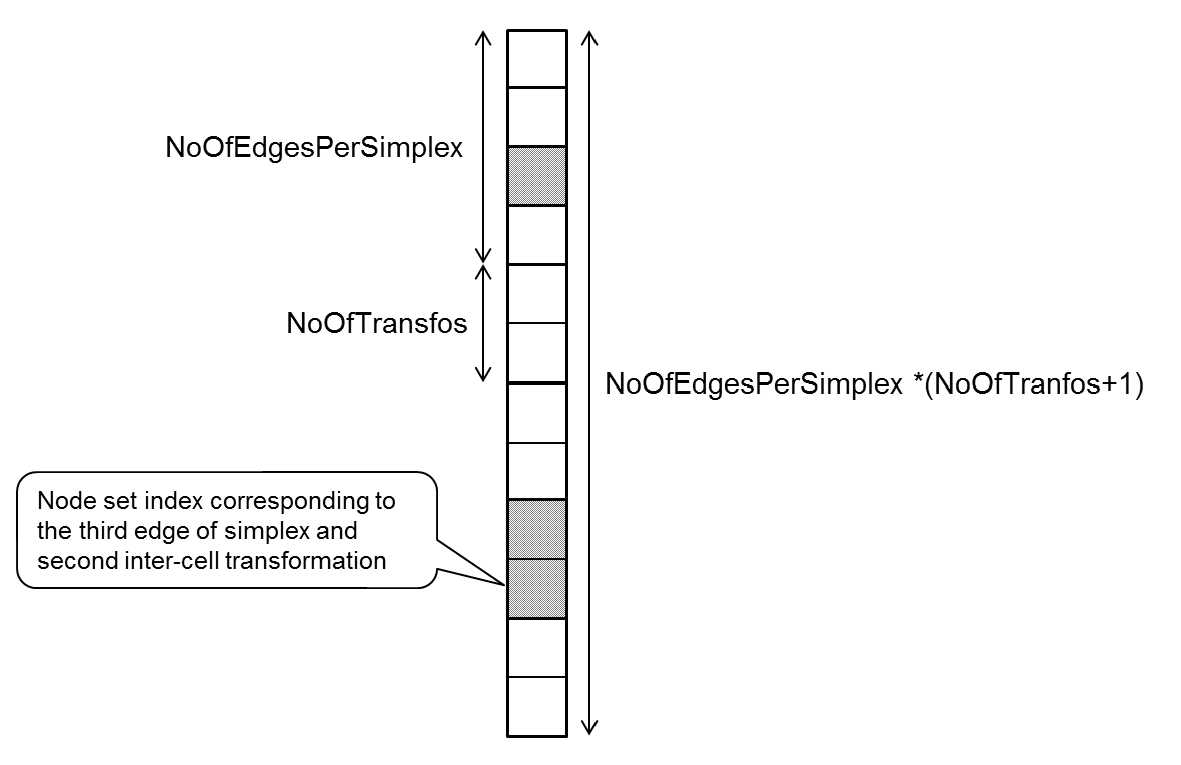
\includegraphics[width=10cm]{Figures/NodeSetFamily}
\end{center}
\caption{Node set family for a nonlinear edge quadrature. For this node set family the volume simplex has four edges and there are two inter cell transformations found for the grid.}
\label{fig:NodeSetFamily}
\end{figure}
\item \textbf{Specifying memory}\\
Besides the memory required for the general quadrature, memory is allocated\coderm{BoSSS.Foundation.Quadrature.NonLin.NECQuadratureEdge.AllocateBuffers(...)} for fields in both neighbors and the required flux values.
\item \textbf{Finding values of test functions}\\
Test functions are found\coderm{BoSSS.Foundation.Quadrature.NonLin.NECQuadratureEdge.PostLockNodes(...)} at the node set family and the values are stored separately at $m\_TestFunctions\_1stCell[e, \gamma][n\_node,m]$ and $m\_TestFunctions\_2ndCell[e, \gamma, k][n\_node,m]$ to distinguish between the test functions of the first and second neighbors.  and $k$ is index for inter cell transformation.
\item \textbf{Evaluation of integrands}\\
For an edge quadrature the integrand is $\hat{n}\cdot \vec{f}_j^* \phi_{jm}$ and $\hat{n}\cdot \vec{f}_j^* \phi_{j'm}$ to be evaluated for both neighbors.
\begin{enumerate}
\item \textbf{Evaluation of all fields}\\
The field values are evaluated at the node set family and stored separately at \\$m\_FieldValuesEdge1[f][i,n\_node]$ and $m\_FieldValuesEdge2[f][i,n\_node]$.
\item \textbf{Transform nodes to global coordinates}\\
Global coordinates $m\_NodesGlobalCoords[i,n\_node,d]$ are found from the nodes $m\_NodesUntransfomedVolCoord\_1stEdge[e][n\_node,d]$.
\item \textbf{Evaluating the numerical fluxes}\\
Numerical fluxes of all equation components of type nonlinear flux corresponding to codomain variable $\gamma$, are calculated for inner edges by \emph{inner edge flux}\coderm{BoSSS.Solution.Utils.NonlinearFlux.InnerEdgeFlux(...)} and for boundary edges by \emph{border edge flux}\coderm{BoSSS.Solution.Utils.NonlinearFlux.BorderEdgeFlux(...)} and accumulated at \\$m\_FluxValues[\gamma][i,n\_node]$.
\item \textbf{Multiplying the numerical fluxes by test functions}\\
Numerical fluxes are multiplied by the scaling factor and the test functions of the first neighbor and added to $EvalResult[i, n\_node, MyMap(\gamma, m)]$ and multiplied by the corresponding values of the second neighbor and subtracted from $EvalResult[i, n\_node, MyMap(\gamma, m)+N_{integrals}]$. That is because the flux considering the second neighbor has the opposite sign with respect to the first neighbor.
\end{enumerate}
\item \textbf{Saving integration results}\\
After integrating (see section \ref{sec:QuadRules}, \nameref{sec:QuadRules}) the quadrature results of an edge quadrature \\$ResultsOfIntegration[i,MyMap(f,m)]$ considering the first neighbor $j$ and \\$ResultsOfIntegration[i,MyMap(f,m)+N_{integrals}]$ considering the second neighbor $j'$ are added to the output of the nonlinear quadrature \\$m\_Output[m\_CodomainMapping.LocalUniqueCoordinateIndex(\gamma, j, m)]$ and \\$m\_Output[m\_CodomainMapping.LocalUniqueCoordinateIndex(\gamma, j', m)]$ respectively.
\end{itemize}


\end{document} 